%\input{/Users/joshyv/Research/misc/latex_paper.tex}
\documentclass{article}
\usepackage{amsmath}
\usepackage{graphicx}
\usepackage{amsfonts}
\usepackage{amssymb}
\usepackage{amsthm}
%\usepackage{cite}
\usepackage{algorithm}
\usepackage{algorithmic}
% \usepackage{times}
\usepackage{fancyhdr}
\usepackage{graphicx}
\usepackage{verbatim}
\usepackage{color}
\usepackage[T1]{fontenc}
\usepackage[scaled]{helvet}
\renewcommand*\familydefault{\sfdefault} %% Only if the base font of the document is to be sans serif
\pagestyle{fancy}

\oddsidemargin=0.0in %%this makes the odd side margin go to the default of 1inch
\evensidemargin=0.0in
\textwidth=6.5in
\headwidth=6.5in
\textheight=9in %%sets the textwidth to 6.5, which leaves 1 for the remaining right margin with 8 1/2X11inch paper
\headheight=12pt
\topmargin=-0.25in
%\headheight=0in
%\headsep=0in
%\pagestyle{headings}

\usepackage{hyperref}
% \usepackage{ulem}
% \usepackage{color}

% \newcommand{\loo}{$L^{(1)}_{h; \mD_n}$}
\newcommand{\conv}{\rightarrow}
% \newcommand{\Real}{\mathbb{R}}
% \providecommand{\tr}[1]{\textcolor{red}{#1}}

\newcommand{\mB}{\mathcal{B}}
\newcommand{\mD}{\mathcal{D}}
\newcommand{\mM}{\mathcal{M}}
\newcommand{\PP}{\mathbb{P}}           % probability
\newcommand{\EE}{\mathbb{E}}           % expected value
\newcommand{\II}{\mathbb{I}}           % expected value
\newcommand{\Real}{\mathbb{R}}           % expected value

\newcommand{\del}{\delta}
\newcommand{\sig}{\sigma}
\newcommand{\lam}{\lambda}
\newcommand{\gam}{\gamma}
\newcommand{\eps}{\varepsilon}

\providecommand{\mc}[1]{\mathcal{#1}}
\providecommand{\mb}[1]{\boldsymbol{#1}}
\providecommand{\mbb}[1]{\mathbb{#1}}
\providecommand{\mv}[1]{\vec{#1}}
\providecommand{\mh}[1]{\widehat{#1}}
\providecommand{\mt}[1]{\widetilde{#1}}
\providecommand{\mhc}[1]{\hat{\mathcal{#1}}}
\providecommand{\mhb}[1]{\hat{\boldsymbol{#1}}}
\providecommand{\mvb}[1]{\vec{\boldsymbol{#1}}}
\providecommand{\mtb}[1]{\widetilde{\boldsymbol{#1}}}

\newcommand{\argmax}{\operatornamewithlimits{argmax}}
\newcommand{\argmin}{\operatornamewithlimits{argmin}}


% \newcommand{\mN}{\mathcal{N}}

\newcommand{\hL}{\widehat{L}}
\newcommand{\MeB}{\mM \overset{\varepsilon}{{\sim}}_{F} \mB}
\newcommand{\MsB}{\mM \overset{S}{\sim}_{F} \mB}
\newcommand{\MnoteB}{\mM \overset{\varepsilon}{{\not\sim}}_{F} \mB}
\providecommand{\tr}[1]{\textcolor{black}{#1}}
\providecommand{\norm}[1]{\left \lVert#1 \right  \rVert}
\newcommand{\T}{^{\ensuremath{\mathsf{T}}}}           % transpose
\newcommand{\from}{\colon}



\newtheorem{defi}{Definition}
\newtheorem{thm}{Theorem}
\newtheorem{thex}{\emph{Gedankenexperiment}}
\lhead{Vogelstein JT, et al.}
\rhead{Statistical Supervenience}


\begin{document}

	\begin{center}
{\huge	Are mental properties supervenient on brain properties?}
\end{center}

\vspace{5px}

\begin{center}
{\large		
Joshua T. Vogelstein$^{1*}$, R. Jacob Vogelstein$^2$, Carey E. Priebe$^1$\\
	$^1$Department of Applied Mathematics \& Statistics, \\ Johns Hopkins University, Baltimore, MD, 21218,\\ $^2$National Security Technology Department, \\ Johns Hopkins University Applied Physics Laboratory, Laurel, MD 20723}
	
\end{center}

\vspace{5px}

% \maketitle
% \date{\vspace{-5ex}}
%\tableofcontents
% \begin{abstract}
	
\noindent The``mind-brain supervenience'' conjecture suggests that all mental properties are derived from the physical properties of the brain. To address the question of whether the mind supervenes on the brain, we frame a supervenience hypothesis in rigorous statistical terms. Specifically, we propose a modified version of supervenience (called $\eps$-supervenience) that is amenable to experimental investigation and statistical analysis. To illustrate this approach, we perform a thought experiment that illustrates how the probabilistic theory of pattern recognition can be used to make a \emph{one}-sided determination of $\eps$-supervenience. The physical property of the brain employed in this analysis is the graph describing brain connectivity (i.e., the brain-graph or connectome). $\eps$-supervenience allows us to determine whether a particular mental property can be inferred from one's connectome to within any given positive misclassification rate, regardless of the relationship between the two. This may provide motivation for cross-disciplinary research between neuroscientists and statisticians.


% \end{abstract}

% \vspace*{0.5 in}

\newpage
% \section*{Introduction}

\noindent Questions and assumptions about mind-brain supervenience go back at least as far as Plato's dialogues in circa 400 BCE \cite{Plato97}.  While there are many different notions of supervenience, we find Davidson's canonical description particularly illustrative \cite{Davidson70}:
%  The mind-brain supervenience notion was canonized in 1970 with the following quote from Donald Davidson \cite{Davidson70}:
\begin{quotation}
\noindent [mind-brain] supervenience might be taken to mean that there cannot be two events alike in all physical respects but differing in some mental respect, or that an object cannot alter in some mental respect without altering in some physical respect.
\end{quotation}
Colloquially, supervenience means ``there cannot be a mind-difference without a physical-difference.''
This philosophical conjecture has potentially widespread implications.  
% We consider a special case of supervenience of considerable interest.  Specifically, this work addresses a version of a local supervenience between mental properties and brain properties, with particular emphasize on brain-graphs (i.e., connectivity structure).  Supervenience questions or assumptions are fundamental to 
% The determination of supervenience (or lack thereof) of minds on brains has potentially important implications in 
% a number of fields of inquiry.  
For example, neural network theory and artificial intelligence often implicitly assume 
a local version mind-brain supervenience \cite{Haykin2008,Ripley2008}. Cognitive neuroscience similarly seems to operate under such assumptions
% , which if falsified, might result in novel perspectives and theories 
\cite{Gazzaniga2008}.  Philosophers continue to debate and refine notions of supervenience 
% And the question of mind-brain supervenience continues to be debated amongst philosophers 
\cite{Kim2007}.  
% Moreover, many cognitive neuroscience investigations could be cast as questions
Yet, to date, relatively scant attention has been paid to what might be empirically learned about supervenience.  

In this work we attempt to bridge the gap between philosophical conjecture and empirical investigations by casting supervenience in a probabilistic framework amenable to hypothesis testing. 
We then use the probabilistic theory of pattern recognition to determine
the limits of what one can and cannot learn about supervenience through data analysis.  
The implications of this work are varied.  It provides a probabilistic framework for converting philosophical conjectures into statistical hypotheses that are amenable to experimental investigation, which  allows the philosopher to gain empirical support for her rational arguments. This leads to the construction of the first explicit proof (to our knowledge) of a universally consistent classifier on graphs, and the first demonstration of the tractability of answering supervenience questions.  Supervenience therefore seems to perhaps be a useful but under-utilized concept for neuroscientific investigations.  This work should provide further motivation for cross-disciplinary efforts across three fields---philosophy, statistics, and neuroscience---with shared goals but mostly disjoint jargon and methods of analysis.






% This work does not attempt to resolve any particular mind-brain supervenience debates.  Rather, we propose a statistical approach for framing mind-brain supervenience questions.  This approach depends on defining the space of mental and brain properties under investigation and a statistical model characterizing the possible distributions governing their relationship.  Such definitions transform supervenience from a conjecture or an assumption into a hypothesis which can be tested.



\section*{Results}

\subsection*{Statistical supervenience: a definition} % (fold)

\noindent Let $\mc{M}=\{m_1, m_2, \ldots\}$ be the space of all possible minds and
let $\mc{B}=\{b_1,b_2,\ldots\}$ be the set of all possible brains.  $\mc{M}$ includes a mind for each possible collection of thoughts, memories, beliefs, etc.
$\mc{B}$ includes a brain for each possible position and momentum of all subatomic particles within the skull.  
Given these definitions, Davidson's conjecture may be concisely and formally stated thusly:  $m \neq m' \implies b \neq b'$, where $(m,b), (m',b') \in \mc{M} \times \mc{B}$ are mind-brain pairs.  This mind-brain supervenience relation does not imply an injective relation, a causal relation, or an identity relation (see Appendix 1 for more details and some examples).  To facilitate both statistical analysis and empirical investigation, we convert this local supervenience relation from a logical to a probabilistic relation.  

% Let $b$ correspond to an agent's brain, which is a particular element from the set of all possible brains, $\mB$. Similarly, let $m$ correspond to an agent's mind, which is a particular element from the set of all possible minds, $\mM$.  
Let $F_{MB}$ indicate a joint distribution of minds and brains. Statistical supervenience can then be defined as follows:
\begin{defi}
\label{def:1} 
$\mM$ is said to \textit{statistically supervene} on $\mB$ for distribution $F=F_{MB}$, denoted $\mM \overset{S}{\sim}_F \mB$, if and only if $\PP[m \neq m' | b=b']=0$, or equivalently $\PP[m = m' | b = b']=1$. 
\end{defi}
\noindent Statistical supervenience is therefore a probabilistic relation on sets which could be considered a generalization of correlation (see Appendix 1 for details).  



\subsection*{Statistical supervenience is equivalent to perfect classification accuracy} % (fold)
\label{sub:theoretical_results}

If minds statistically supervene on brains, then if two minds differ, there must be some brain-based difference to account for the mental difference.  This means that there must exist a deterministic function $g^*$ mapping each brain to its supervening mind. One could therefore, in principle, know this function. When the space of all possible minds is finite---that is, $|\mM| < \infty$---any function $g\from \mB \to \mM$ mapping from minds to brains is called a \emph{classifier}.  
% Let $\mh{m}$ denote the output of a classifier, $g(b)=\mh{m}$.  
Define misclassification rate, the probability that $g$ misclassifies $b$ under distribution $F=F_{MB}$,  as
\begin{align} \label{eq:1}
L_{F}(g) = \PP[g(B) \neq M] =  \sum_{(m,b) \in \mc{M} \times \mc{B}} \II\{g(b) \neq m\} \PP[B=b, M=m],	
\end{align}
where $\II\{\cdot\}$ denotes the indicator function taking value unity whenever its argument is true and zero otherwise.  The Bayes optimal classifier $g^*$ minimizes $L_{F}(g)$ over all classifiers:	
$g^* = \argmin_{g} L_{F}(g)$.
The \emph{Bayes error}, or Bayes risk, $L^*=L_{F}(g^*)$, is the minimum possible misclassification rate.

% The optimal such classifier, $g^*$, has the smallest expected misclassification rate, $L^*=L_{F}(g^*)$, under distribuion $F$.  The minimum misclassification rate is called Bayes error (see Methods for details). 
The primary result of casting supervenience in a statistical framework is the below theorem, which 
follows immediately from Definition \ref{def:1} and Eq. \eqref{eq:1}: 
\begin{thm}
\label{thm:1} 
% $\mM$ is said to \textit{statistically supervene} on $\mB$ for distribution $F=F_{MB}$, denoted 
$\mM \overset{S}{\sim}_{F} \mB \Leftrightarrow L^*= 0$.
 %Formally, \mbox{$\MsB \Leftrightarrow L^*=0$}.  
\end{thm}
% \begin{proof}
% Let $\mc{M}_b=\{m: \PP[B=b | M=m] >0\}$.  
% $$L^*=0 \Leftrightarrow |\mc{M}_b|=1 \, \forall \, b\in \mc{B} : \PP[B=b]>0. $$
% In words, for $L^*$ to equal 0, it must be the case that there exists only a single $m$ for each $b$.
% \end{proof}

% \noindent If minds supervene on brains, then, by the definition of supervenience, there exists a function that maps each brain deterministically to a particular mind.  This means that one could draw a decision boundary between all equivalence classes of brains, each class corresponding to a different mind, and no mind will reside within two different equivalence classes.  Thus, the optimal classifier would correctly find these decision boundaries, and therefore have no opportunity to err. $\square$

The above argument shows (for the first time to our knowledge) that statistical supervenience and zero Bayes error are equivalent. Statistical supervenience can therefore be thought of as a constraint on the possible distributions on minds and brains.  Specifically, let $\mc{F}$ indicate the set of all possible joint distributions on minds and brains, and let $\mc{F}_s = \{F_{MB} \in \mc{F}: L^*=0\}$ be the subset of distributions for which supervenience holds. Theorem \ref{thm:1} implies that $\mc{F}_s  \subsetneqq \mc{F}$.  Mind-brain supervenience is therefore an extremely restrictive assumption about the possible relationships between minds and brains.  It seems that such a restrictive assumption begs for empirical evaluation, vis-\'a-vis, for instance, a hypothesis test.


\subsection*{The non-existence of a viable statistical test for supervenience} % (fold)
\label{sub:subsection_name}

% subsection subsection_name (end)

The above theorem implies that if we desire to know whether  minds supervene on brains, we can check whether $L^*=0$.  Unfortunately, $L^*$ is typically unknown.  Fortunately, we can approximate $L^*$ using training data.

Assume that training data $\mc{T}_n=\{(M_{1},B_{1}), \ldots, (M_{n},B_{n})\}$ are each sampled identically and independently (iid) from the true (but unknown) joint distribution $F=F_{MB}$.  Let $g_n$ be a classifier induced by the training data, $g_n:\mB \times (\mc{M} \times \mc{B})^n \mapsto \mM$.  The  misclassification rate of such a classifier is given by
\begin{align}
L_F(g_n)=\sum_{(m,b)  \in \mc{M}\times \mc{B}} \II\{g_n(b; \mc{T}_n) \neq m\} \PP[B=b,M=m],
\end{align}
%  The expected misclassification rate is given by 
% \begin{align}
% \EE[L_F(g_n)]=\sum_{(m,b)  \in \mc{M}\times \mc{B}} \II\{g_n(b; \mc{T}_n) \neq m\} \PP[B=b,M=m],
% \end{align}
which is a random variable due to the dependence on a randomly sampled training set $\mc{T}_n$.  
% where the expectation is taken with respect to the training data $\mc{T}_n$. 
Calculating the expected misclassification rate $\EE[L_F(g_n)]$ is often intractable in practice because it requires a sum over all possible training sets.  Instead, expected misclassification rate can be approximated by ``hold-out'' error.  Let $\mc{H}_{n'}=\{(M_{n+1},B_{n+1}), \ldots, (M_{n+n'},B_{n+n'})\}$ be a set of $n'$ hold-out samples, each sampled iid from $F_{MB}$.  The hold-out approximation to the misclassification rate is given by
\begin{align}
\hL^{n'}_{F}(g_{n}) = \sum_{(M_i,B_i) \in \mc{H}_{n'}}\II \{g_{n}(B_i; \mc{T}_{n})\neq M_i\} \approx \EE[L_F(g_n)] \geq L^*. % \PP[B=b,M=m].	
\end{align}
% Under the above assumptions, $\hL^{n'}_F(g_n)$ 
% which can be used as a surrogate for $L^*$. 
By definition of $g^*$, the expectation of $\hL^{n'}_F(g_n)$ (with respect to both $\mc{T}_n$ and $\mc{H}_{n'}$)  is greater than or equal to $L^*$ for any $g_n$ and all $n$.  Thus, we can construct a hypothesis test for $L^*$ using the surrogate $\hL^{n'}_F(g_n)$.  

A statistical test proceeds by 
specifying the allowable Type I error rate $\alpha>0$ and then
calculating a 
test statistic.
The $p$-value---the probability of rejecting the least favorable null hypothesis (the simple hypothesis within the potentially composite null which is closest to the boundary with the alternative hypothesis)---is the probability of observing a result at least as extreme as the observed.  In other words, the $p$-value is the cumulative distribution function of the test statistic evaluated at the observed test statistic with parameter given by the least favorable null distribution.
% a functional of the distribution of the test statistic.  
% and a critical value $c_\alpha$.  
We reject if 
% the test statistic is more extreme than the critical value, or equivalently, if 
the $p$-value 
is less than $\alpha$.   A test is \emph{consistent} whenever its power  (the probability of rejecting the null when it is indeed false)  goes to unity as $n\conv \infty$ . For any statistical test, if the $p$-value converges in distribution to $\delta_0$ (point mass at zero), then whenever $\alpha >0$, power goes to unity. 

% Ideally, 
Based on the above considerations,
we might consider the following hypothesis test: $H_0: L^*>0$ and $H_A: L^*=0$; rejecting the null indicates that $\MsB$. Unfortunately, 
% because the null hypothesis is not closed, 
the alternative hypothesis lies on the boundary, so the $p$-value is always equal to unity \cite{Bickel2000}.  From this, Theorem \ref{thm:2} follows immediately:
\begin{thm} \label{thm:2}
	There does not exist a viable test of $\MsB$.
\end{thm}

In other words, we can \emph{never} reject $L^*>0$ in favor of supervenience, no matter how much data we obtain.  

\subsection*{Conditions for a consistent statistical test for $\eps$-supervenience} % (fold)


To proceed, therefore, we introduce a relaxed notion of supervenience: 
% Let $\MeB$ denote that $\mc{M}$ is $\eps$-supervenient on $\mc{B}$ for distribution $F=F_{MB}$, for $\eps>0$.  We define $\MeB$ as follows:
\begin{defi}
\label{def:2}
$\mM$ is said to $\eps$-\textit{supervene} on $\mB$ for distribution $F=F_{MB}$, denoted $\MeB$, if and only if $L^*< \eps$ for some $\eps>0$.
% $$\MeB \Leftrightarrow L^*< \eps.$$
% Given $\varepsilon > 0$, $\mM$ is said to $\varepsilon$-\textit{supervene} on $\mB$ for distribution $F=F_{MB}$ if and only if $L_F(g^*)< \eps$. 
%, denoted $\MeB \Leftrightarrow L_{F}(g^*) < \varepsilon$.
\end{defi}
\noindent 
% For brevity, let $\MeB$ denote that $\mc{M}$ is $\eps$-supervenient on $\mc{B}$ 
Given this relaxation, consider the problem of testing for $\eps$-supervenience:
\begin{align*}
	H_0^{\eps}: L^* \geq \eps \\
	H_A^{\eps}: L^* < \eps.
\end{align*}
Let $\mh{n}= n' \hL^{n'}_{F}(g_n)$ be the \emph{test statistic}. 
The distribution of $\mh{n}$ is available under the least favorable null distribution. 
% to the alternative hypothesis.  
% The $p$-value is given by the least favorable null distribution to the alternative hypothesis.
For the above hypothesis test,  
% for this hypothesis test 
the $p$-value is therefore the binomial cumulative distribution function with parameter $\eps$; that is, $p$-value $=\mathbb{B}(\mh{n}; n', \eps)= \sum_{k \in [\mh{n}]_0}$Binomial$(k; n'; \eps)$, where
% Let 
% and
$[\mh{n}]_0=\{0,1,\ldots, \mh{n}\}$.  We reject whenever this $p$-value is less than $\alpha$; rejection implies that we are $100(1-\alpha$)\% confident that $\MeB$.   

 For the above $\eps$-supervenience statistical test, if $g_n \conv g^*$ as $n \conv \infty$, then $\hL^{n'}_F(g_n) \conv L^*$ as $n,n' \conv \infty$.  Thus, if $L^* < \eps$, 
power goes to unity.
% the $p$-value converges; that is, $\mathbb{B}(\mh{n}; n', \eps) \conv \delta_0$.
The definition of $\eps$-supervenience therefore admits, for the first time to our knowledge, a viable statistical test of supervenience, given a specified $\eps$ and $\alpha$. Moreover, this test is consistent whenever $g_n$ converges to the Bayes classifier $g^*$.





\subsection*{The existence and construction of a consistent statistical test for $\eps$-supervenience} % (fold)
\label{sub:uc}

The above considerations indicate the existence of a consistent test for $\eps$-supervenience whenever the classifier used is consistent.  
% that to construct a statistical test with guaranteed limiting unity power, a universally consistent classifier (one for which $\hL^{n'}_F(g_n) \conv L_F(g^*)$ as $n,n' \conv \infty$) is required. 
To actually implement such a test, one must be able to (i) measure mind/brain pairs and (ii) have a consistent classifier $g_n$.  Unfortunately, we do not know how to measure the entirety of one's brain, much less one's mind. 
% Moreover, even if we did, we do not know the joint distribution of mind/brain pairs, $F_{MB}$.  
We therefore must restrict our interest to a mind/brain \emph{property} pair.  
A mind (mental) property might be a person's intelligence, psychological state, current thought, gender identity, etc.  A brain property might be the number of cells in a person's brain at some time $t$, or the collection of spike trains of all neurons in the brain during some time period $t$ to $t'$.  Regardless of the details of the specifications of the mental property and the brain property, given such specifications, one can assume a model, $\mc{F}$.  We desire a classifier $g_n$ that is guaranteed to be consistent, no matter which of the possible distributions $F_{MB} \in \mc{F}$ is the true distribution.  A classifier with such a property is called a \emph{universally consistent classifier}.  
Below, under a very general mind-brain model $\mc{F}$, we construct a universally consistent classifier. 
% is readily available.


% To ensure consistency and therefore unity power, the classifier $g_n$ must be able to converge to the truth, regardless of the true distribution, $F$.  We therefore make explicit a model for brains, and show that under this very general model, universally consistent classifiers are available.

\begin{thex} \label{exp:1}
Let the physical property under consideration be brain connectivity structure, so $b$ is a brain-graph (``connectome'') with vertices representing neurons (or collections thereof) and edges representing synapses (or collections thereof). Further let $\mB$, the brain observation space, be the collection of all graphs on a given finite number of vertices, and let $\mc{M}$, the mental property observation space, be finite. Now, imagine collecting very large amounts of very accurate identically and independently sampled  brain-graph data and associated mental property indicators from $F_{MB}$. A $k_n$-nearest neighbor classifier using a Frobenius norm is universally consistent (see Methods for details). 
% Therefore, %Theorem \ref{thm:1} applies and 
The existence of a universally consistent classifier guarantees that eventually (in $n,n'$) we will be able to conclude $\MeB$ for this mind-brain property pair, if indeed $\varepsilon$-supervenience holds. This logic holds for directed graphs or multigraphs or hypergraphs with discrete edge weights and vertex attributes, as well as unlabeled graphs (see \cite{VP11_unlabeled} for details). Furthermore, the proof holds for other matrix norms (which might speed up convergence and hence reduce the required $n$), and the regression scenario where $|\mM|$ is infinite (again, see Methods for details).  
\end{thex}
Thus, under the conditions stated in the above \emph{Gedankenexperiment}, universal consistency yields:
\begin{thm} \label{thm:3}
	$\MeB \implies \beta \conv 1$ as $n,n'\conv \infty$.
\end{thm}


Unfortunately, the rate of convergence of $L_{F}(g_n)$ to $L_{F}(g^*)$ depends on the (unknown) distribution $F=F_{MB}$ \cite{DGL96}. Furthermore, arbitrarily slow convergence theorems regarding the rate of convergence of $L_{F}(g_n)$ to $L_{F}(g^*)$ demonstrate that there is no universal $n,n'$ which will guarantee that the test has power greater than any specified target $\beta > \alpha$ \cite{Devroye83}. For this reason, the test outlined above can provide only a one-sided conclusion: if we reject we can be $100(1-\alpha)$\% confident that $\MeB$ holds, but we can never be confident in its negation; rather, it may be the case that the evidence in favor of $\MeB$ is insufficient 
% for any number of reasons, including that 
because we simply have not yet collected enough data. 
% Thus, without restrictions on $F_{MB}$, arbitrarily slow convergence theorems imply that our theorem of $\varepsilon$-supervenience does not \tr{strictly} satisfy Popper's {\it falsifiability} requirement \cite{Popper}.
This leads immediately to the following theorem:
\begin{thm} \label{thm:4}
For any target power $\beta_{min} > \alpha$, there is no universal $n,n'$ that guarantees $\beta \geq \beta_{min}$.
\end{thm}

% Moreover, switching the null and alternative hypotheses---yielding $H_0^{\eps'}: L^*<\eps$ and $H_A^{\eps'}: L^* \geq \eps$---does not resolve the matter.
Therefore, even $\eps$-supervenience does not satisfy Popper's falsifiability criterion \cite{Popper1959}.


\subsection*{The feasibility of a consistent statistical test for $\eps$-supervenience} % (fold)


Theorem \ref{thm:3} demonstrates the availability of a consistent test under certain restrictions.  Theorem \ref{thm:4}, however, demonstrates that convergence rates might be unbearably slow.  We therefore provide an illustrative example of the feasibility of such a test on synthetic data.

{\it Caenorhabditis elegans} is a species whose nervous system is believed to consist of the same $279$ labeled neurons for each organism \cite{Durbin87}. Moreover, these animals exhibit a rich behavioral repertoire that seemingly depends on circuit properties \cite{deBonoMaricq05}.  These findings motivate the use of C.~elegans for a synthetic data analysis \cite{GelmanShalizi11}.  Conducting such an experiment requires specifying a joint distribution $F_{MB}$ over brain-graphs and behaviors.  The joint distribution decomposes into the product of a class-conditional distribution (likelihood) and a prior, $F_{MB}=F_{B|M}F_M$. The prior  specifies the probability of any particular organism exhibiting the behavior.  The class-conditional distribution specifies the brain-graph distribution given that the organism does (or does not) exhibit the behavior. 

Let $A_{uv}$ be the number of chemical synapses between neuron $u$ and neuron $v$ according to \cite{VarshneyChklovskii09}.  Then, let $\mc{S}$ be the set of edges deemed responsible for odor-evoked behavior according to \cite{ChalasaniBargmann07}.  If odor-evoked behavior is supervenient on this signal subgraph $\mc{S}$, then the distribution of edges in $\mc{S}$ must differ between the two classes of odor evoked behavior \cite{VP11_sigsub}.  Let $E_{uv|j}$ denote the expected number of edges from vertex $v$ to vertex $u$ in class $j$.   For class $m_0$, let $E_{uv|0}=A_{uv}+\eta$,  where $\eta=0.05$ is a small noise parameter  (it is believed that the C.~elegans connectome is similar across organisms \cite{Durbin87}). For class $m_1$, let $E_{uv|1}=A_{uv}+z_{uv}$, where the signal parameter $z_{uv}=\eta$ for all edges not in $\mc{S}$, and $z_{uv}$ is uniformly sampled from $[-5,5]$ for all edges within $\mc{S}$. For both classes, let each edge be Poisson distributed, $F_{A_{uv}|M=m_j}$= Poisson$(E_{uv|j})$.
% Let the mental property correspond to the C.~elegans exhibiting (or not exhibiting) a particular behavior (e.g., response to an odor).  Thus, one can specify $F_{M=m_1}$ and $F_{M=m_0}$, the probability of a C.~elegans exhibiting or not a particular behavior.   The class-conditional distributions $F_{B|M=m_j}$ are therefore the distributions of brain-graphs conditional on whether the C.~elegans exhibits said property.

% Now, to generate the data, let $E_{uv|j}$ be an integer-valued random variable whose value indicates the number of chemical synapses (edges) between neurons (vertices) $u$ and $v$ for class $j$. 

We consider $k_n$-nearest neighbor classification of labeled multigraphs (directed, with loops) on 279 vertices, under Frobenius norm. The $k_n$-nearest neighbor classifier used here satisfies $k_n \rightarrow \infty$ as $n \rightarrow \infty$ and $k_n/n \rightarrow 0$ as $n \rightarrow \infty$, ensuring universal consistency. (Better classifiers can be constructed for the joint distribution $F_{MB}$ used here; however, we demand universal consistency.)  Figure \ref{fig:1} shows that for this simulation, rejecting $(\eps=0.1)$-supervenience at $\alpha=0.01$ requires only a few hundred training samples.


% Simulations suggest that one may build a classifier, practically and with a manageable training sample size $n$, that demonstrates $\varepsilon$-supervenience with reasonable choices for $\varepsilon$ and $\alpha$, and a plausible joint distribution $F_{MB}$ (Figure \ref{fig:1}). 



\begin{figure}[!ht]
\centering 
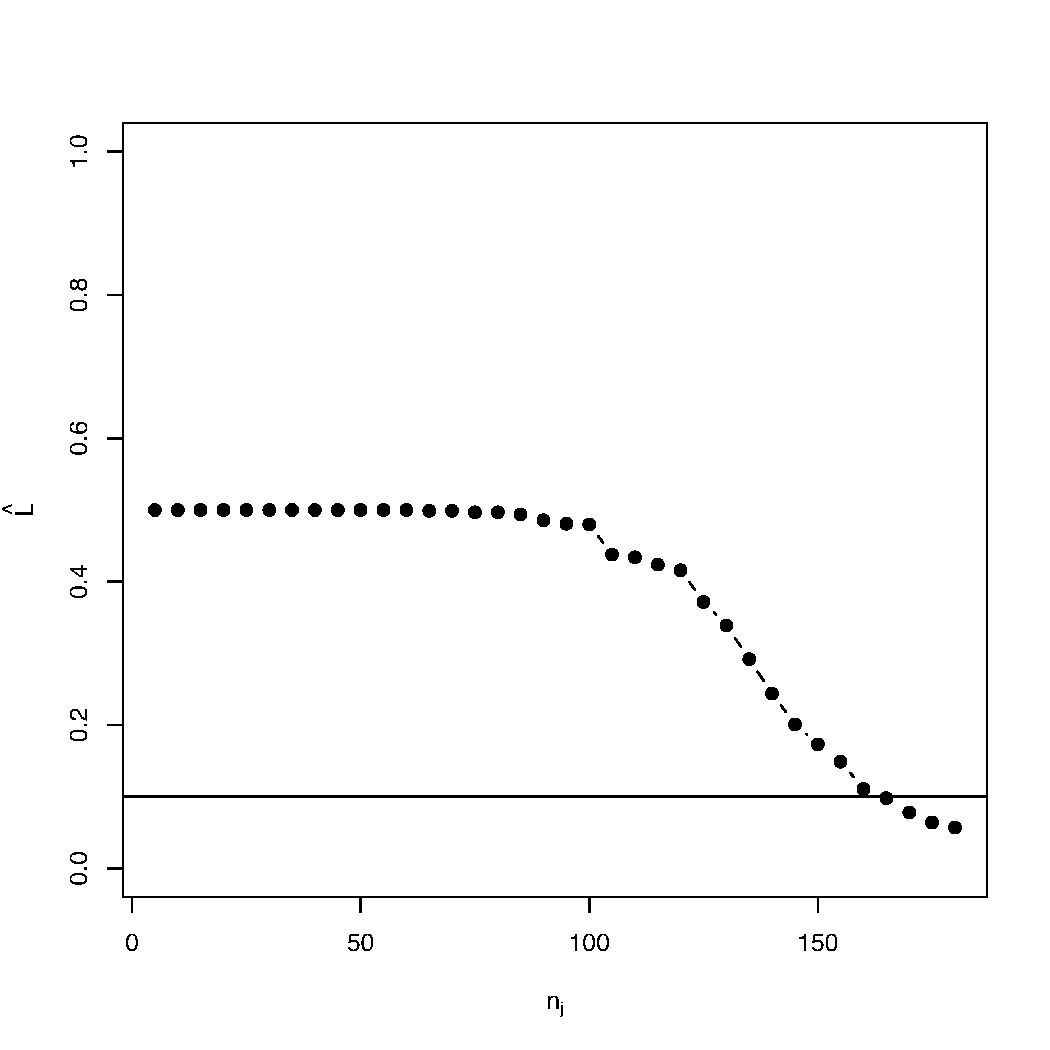
\includegraphics[width=.5\linewidth]{Lhatplot}
\caption{C.~elegans graph classification simulation results.  The estimated hold-out misclassification rate $\hL^{n'}_{F}(g_{n})$  (with $n'=1000$ testing samples) %$\hL^{1000}_{\PP}(g_{\mt{n}})$ 
is plotted as a function of class-conditional training sample size $n_j=n/2$, suggesting that for $\varepsilon=0.1$ we can determine that $\MeB$ holds with $99\%$ confidence with just a few hundred training samples generated from $F_{MB}$. Each dot depicts $\hL^{n'}_{F}(g_n)$ for some $n$; standard errors are $(\hL^{n'}_{F}(g_{n}) (1-\hL^{n'}_{F}(g_{n}))/n')^{1/2}$.  For example, at $n_j = 180$ we have $k_n = \lfloor\sqrt{8 n}\rfloor=53$ (where $\lfloor\cdot\rfloor$ indicates the floor operator), $\hL^{n'}_{F}(g_{n}) = 0.057$, and standard error less than $0.01$. We reject $H_0^{0.1}: L^* \geq 0.1$ at $\alpha=0.01$. Note that $L^* \approx 0$ for this simulation.}
\label{fig:1}
\end{figure}

Importantly, conducting this experiment {\it in actu} is not beyond current technological limitations. 3D superresolution imaging \cite{Vaziri2008} combined with neurite tracing algorithms \cite{Helmstaedter2008,Mishchenko09,LuLichtman09} allow the collection of a C. elegans brain-graph within a day. Genetic manipulations, laser ablations, and training paradigms can each be used to obtain a non-wild type population for use as $M=m_1$ \cite{deBonoMaricq05}, and the class of each organism ($m_0$ vs.~$m_1$) can also be determined automatically \cite{Buckingham2008}.





\section*{Discussion}

% \paragraph{Summary} % (fold)
% \label{par:summary}

This work makes the following contributions.  First, we define statistical supervenience based on Davidson's canonical statement (Definition \ref{def:1}).  This definition makes it apparent that supervenience implies the possibility of perfect classification (Theorem \ref{thm:1}).  
We then prove that there is no viable test against supervenience, so one can \emph{never} reject a null hypothesis in favor of supervenience, regardless of the amount of data (Theorem \ref{thm:2}).  This motivates the introduction of a relaxed notion called $\eps$-supervenience (Definition \ref{def:2}), against which consistent statistical tests are readily available. Under a very general brain-graph/mental property model (\emph{Gedankenexperiment} \ref{exp:1}),  a consistent statistical test against $\eps$-supervenience is always available no matter the true distribution $F_{MB}$ (Theorem \ref{thm:3}).  
In other words, the proposed test is guaranteed to reject the null whenever the null is false, given sufficient data, for any possible distribution governing mental property/brain property pairs. 

Alas, arbitrary slow convergence theorems demonstrate that there is no universal $n,n'$ for which convergence is guaranteed (Theorem \ref{thm:4}).  Thus, a failure to reject is ambiguous: even if the data satisfy the above assumptions, the failure to reject may be due to either (i) an insufficient amount of data or (ii) $\mc{M}$ may not be $\eps$-supervenient on $\mc{B}$.  Moreover, the data will not, in general, satisfy the above assumptions.  In addition to dependence (because each human does not exist in a vacuum), the mental property measurements will often be ``noisy'' (for example, accurately diagnosing psychiatric disorders is a sticky wicket \cite{Kessler2005}). 
% has a number of possible explanations.  First, the amount of data might be insufficient; collecting more data or utilizing a more informative distance might resolve this difficulty.  Second, the class labels (mental property indicators) may not be faithful representations of the mental property of interest (mental property observations may be ``noisy'' indicators). 
% 
% Second, it may be that the mental property under investigation is supervenient to a different brain property.  
% Third,  Fourth, the mental property may really not be supervenient to any brain properties (although testing this more global notion of supervenience is not possible, as one can never be sure that one as measured all brain properties).  
Nonetheless, synthetic data analysis suggests that under somewhat realistic assumptions, convergence obtains with an amount of data one might conceivably collect (Figure \ref{fig:1} and ensuing discussion).  


 

% We have introduced the notion of $\eps$-supervenience, which states that the Bayes optimal misclassification rate for any mind-brain property pair is less than $\eps$.  This definition admits, for the first time to our knowledge, a viable statistical test for supervenience.  Furthermore, when we restrict the space of minds and brains to the setting of \emph{Gedankenexperiment}  1, we have shown that $k_n$-NN classifiers are universally consistent, such that one can derive a hypothesis test, with confidence level $\alpha$, that is guaranteed to converge to the Bayes optimal misclassification rate, given sufficient data, no matter the true (but unknown) distribution of mind-brain pair properties.  

 %one can never determine the reason for a failure to reject. %one can never determine whether (i) more data is necessary to get a lower p-value, or (ii) that the particular $\eps$-supervenience does not hold.  

% Second, $\eps$-supervenience is defined between a mental property and a brain property.  Thus, a failure to reject $\eps$-supervenience on a particular brain property does not entail non-$\eps$-supervenience on any other brain property.  Third, in general, neither mental properties nor brain properties are directly measurable; rather, one typically measures a function of such properties.  For instance, instead of measuring intelligence, one may consider the results of an IQ test as a proxy for intelligence. 

 % Similarly, instead of measuring neural spike trains, one estimates spike trains from some measurable neural signal, like voltage.  While one could conceivably ask questions such as: ``is IQ score at some time supervenient on the the output of a voltage measuring device?'', these are less elegant and general than their non-observable analogs, such as: ``is intelligence supervenient on spike trains?''

Thus, given measurements of mental and brain properties that we believe reflect the properties of interest, and given a sufficient amount of data satisfying the independent and identically sampled assumption, a rejection of $H_0^{\eps}: L^*\geq \eps$ in favor of $\MeB$ entails that we are $100(1-a)\%$ confident that the mental property under investigation is $\eps$-supervenient on the brain property under investigation.  Unfortunately, failure to reject is more ambiguous. 
% $\eps-$supervenience tests can therefore be thought of as constraining the space of possible brain properties upon which a mental property supervenes.  
% Determining that a mental property does not supervene on \emph{any} brain property is beyond the capacities of this formalism.

Interestingly, much of contemporary research in neuroscience and cognitive science could be cast as mind-brain supervenience investigations.  Specifically, searches for ``engrams'' of  memory traces \cite{Lashley50} or ``neural correlates''  of various behaviors or mental properties (for example, consciousness \cite{Koch2010}), may be more aptly called searches for the ``neural supervenia'' of such properties.
Letting the brain property be a brain-graph is perhaps especially pertinent in light of the advent of ``connectomics'' \cite{SpornsKotter05,Hagmann05}, a field devoted to estimating whole organism brain-graphs and relating them to function.  Testing supervenience of various mental properties on these brain-graphs will perhaps therefore become increasingly compelling; the framework developed herein could be fundamental to these investigations.  
For example, questions about whether connectivity structure alone is sufficient to explain a particular mental property is one possible mind-brain $\eps$-supervenience investigation.  The above synthetic data analysis demonstrates the feasibility of $\eps$-supervenience on small brain-graphs.
Note that $\eps$-supervenience tests need not investigate seemingly intractable problems, like consciousness.  For example, aspects of visual perception appear to supervene on visual cortical activity (for example, binocular rivalry \cite{Tong2006}). Moreover, an inability to reject $\eps$-supervenience for small $\eps$ is also potentially meaningful.  For example, perhaps auditory localization precision supervenes on a rate code only to some $\eps > c$, the rest supervening on a spike timing code \cite{Chase2006}. 
Similar supervenience tests on increasingly complex mental properties will potentially benefit from either higher-throughput imaging modalities \cite{HayworthLichtman06, Bock2011}, more coarse brain-graphs \cite{PalmAmunts10,Johansen-Berg2009}, or both.




% \paragraph{Human applications} % (fold)
% \paragraph{Dynamics vs. statics} % (fold)
% \paragraph{Concluding thoughts} % (fold)
% \label{par:concluding_thoughts}

% In conclusion, this \emph{Gedankenexperiment}, together with (i) the formal definition of $\varepsilon$-supervenience as a constraint on distributions, (ii) the brain-graph model, and (iii) the universal consistency proof on graphs, is the first demonstration (to our knowledge) that empirically investigating supervenience is at least theoretically possible. The above discussion suggests that many previously conducted investigations either assume supervenience, or try to test it.  Further, new technologies facilitate testing supervenience of mental properties on brain-graphs more easily.


\section*{Methods}
\label{sec:methods}



% Consider the following problem setup.  We have a collection of training data, $\mc{T}_n =\{(m_i,b_i)\}_{i=1}^n$, each sampled exchangeably from some unknown joint distribution, $(m_i,b_i)\sim F_{MB}$, where $m_i$ and $b_i$ are the observed mental and brain properties of experiment $i$, respectively.  A new brain, $b$, called the ``test brain'', is then observed, and one desires to find the most likely class of the new brain, $m$.  It is further assumed that the test mind-brain pair is sampled from the same distribution as the training data, $(m,b)\sim F_{MB}$, and $m$ is unobserved. Further assume that $m$ can take one of a finite number of possible values, that is, $|\mc{M}|<\infty$, and that  $\mc{B}$ is countable.

The $1$-nearest neighbor ($1$-NN) classifier works as follows.  Compute the distance between the test brain  $b$ and all $n$ training brains, $d_i=d(b,b_i)$ for all $i \in [n]$, where $[n]=1,2,\ldots, n$.  Then, sort these distances, $d_{(1)} < d_{(2)} < \ldots < d_{(n)}$, and consider their corresponding minds, $m_{(1)}, m_{(2)}, \ldots, m_{(n)}$, where parenthetical indices indicate rank order among $\{d_i\}_{i\in[n]}$.  %One can then also obtain a rank order for the training minds, $m_{(1)}, m_{(2)}, \ldots, m_{(n)}$, where $m_{(i)}$ is the class of the $i^{th}$ closest training brain to $b$.  
The $1$-NN algorithm predicts that the unobserved mind is of the same class as the closest brain's class: $\mh{m}=m_{(1)}$.  The $k_n$ nearest neighbor is a straightforward generalization of this approach.  It says that the test mind is in the same class as whichever class is the plurality class among the $k_n$ nearest neighbors, $\mh{m}=\argmax_{m'}\II\{\sum_{i=1}^{k_n} m_{(i)}=m'\}$.  Given a particular choice of $k_n$ (the number of nearest neighbors to consider) and a choice of $d(\cdot,\cdot)$ (the distance metric used to compare the test datum and training data), one has a relatively simple and intuitive algorithm.  

Let $g_n$ be the $k_n$ nearest neighbor ($k_n$NN) classifier when there are $n$ training samples.  
A collection of such classifiers $\{g_n\}$,  with $k_n$ increasing with $n$, is called a classifier sequence.  
A universally consistent classifier sequence is any classifier sequence that is guaranteed to converge to the Bayes optimal classifier regardless of the true distribution from which the data were sampled; that is, a universally consistent classifier sequence satisfies $L_F(g_n) \conv L_F(g^*)$ as $n \conv \infty$ for all $F_{MB}$. In the main text, we refer to the whole sequence as a classifier.

% In particular, as $n$ increases, $k_n$ must also increase, but not quite as quickly.  Formally, $k_n$ must satisfy
The $k_n$NN classifier is consistent if (i) $k_n \conv \infty$ as $n \conv \infty$ and (ii) $k_n/n \conv 0$ as $n\conv\infty$ \cite{Stone1977}. In Stone's original proof \cite{Stone1977}, $b$ was assumed to be a $q$-dimensional vector, and the $L_2$ norm ($d(b,b')=\sum_{j=1}^q (b_j-b_j')^2$, where $j$ indexes elements of the $q$-dimensional vector) was shown to satisfy the constraints on a distance metric for this collection of classifiers to be universally consistent.  Later, others extended these results to apply to any $L_p$ norm \cite{DGL96}.  When brain-graphs are represented by their adjacency matrices, one can stack the columns of the adjacency matrices, effectively embedding graphs into a vector space, in which case Stone's theorem applies.  Stone's original proof also applied to the scenario when $|\mc{M}|$ was infinite, resulting in a universally consistent regression algorithm as well.

Note that the above extension of Stone's original theorem to the graph domain implicitly assumed that vertices were labeled, such that elements of the adjacency matrices could easily be compared across graphs.  In theory, when vertices are unlabeled, one could first map each graph to a quotient space invariant to isomorphisms, and then proceed as before.  Unfortunately, 
there is no known polynomial time complexity algorithm for graph isomorphism
% solving the graph-matching problem is currently NP-Incomplete (meaning it is not known to be either P or NP) 
\cite{GareyJohnson79}, so in practice, dealing with unlabeled vertices will likely be computationally challenging \cite{VP11_unlabeled}.



% \subsection*{Supervenience} % (fold)
% \label{sec:preliminaries}

% \subsection*{Mind Brain Supervenience} % (fold)
% \label{sub:supervenience}

% subsection supervenience (end)
% The intention in this work is to develop greater insight regarding the relationship between minds and brains, using statistical methods, with particular interest in notions of supervenience.  Modern philosophy of science suggests that adequate scientific explanations must account for the objects of investigation and their relationships \cite{Craver07}. Therefore, here we define minds, brains, and supervenience.
% The mind-brain supervenience conjecture is a relation between the set of mental states and the set of brain states.  


% \subsection*{Statistical Setting} % (fold)

% The approximate  number of misclassified minds therefore has a binomial distribution:  $n' \hL^{n'}_{F}(g_{n}) \sim \text{Binomial}(n',L_{F}(g_{n}))$.




\clearpage
\bibliography{/Users/jovo/Research/latex/library}
\bibliographystyle{nature}

\section*{Acknowledgments}

The authors would like to acknowledge helpful discussions with J.~Lande, B.~Vogelstein, S.~Seung, and K.~Kording.

\section*{Author Contributions}

JTV, RJV, and CEP conceived of the manuscript.  JTV and CEP wrote it.  CEP ran the experiment.

\section*{Additional Information}

The authors have no competing financial interests to declare.





\end{document}

